\chapter{Deep Learning}

\section{Convolutional Neural Networks}

Convolutional Neural Networks are a specialized kind of neural network for processing data with a known, grid-like topology, such as 2D images. The name ``convolutional'' refers to the usage of the mathematical operation called \textbf{convolution}, indicated by an asterisk ($*$). This is an operation of two functions of a real valued argument, defined as follows:
\begin{equation*}
    s(t) = (f * g)(t) \stackrel{def}{=} \int_{-\infty}^{\infty} f(\tau)g(t - \tau) d \tau = \int_{-\infty}^{\infty} f(t - \tau)g(\tau) d\tau \,,
\end{equation*}
The idea behind this operator is that we want to calculate the average of $f$ weighted by another function $g$ moved over time (``sliding''), calculated for a certain $\tau$. In convolutional network terminology, the first argument (here, $f$) is referred to as the \textbf{input}, and the second argument ($g$) as the \textbf{kernel}. The output is called \textbf{feature map}.

This operator can be applied to neural networks as well. Consider a simple network with one hidden layer:
\begin{figure}[h]
    \centering
    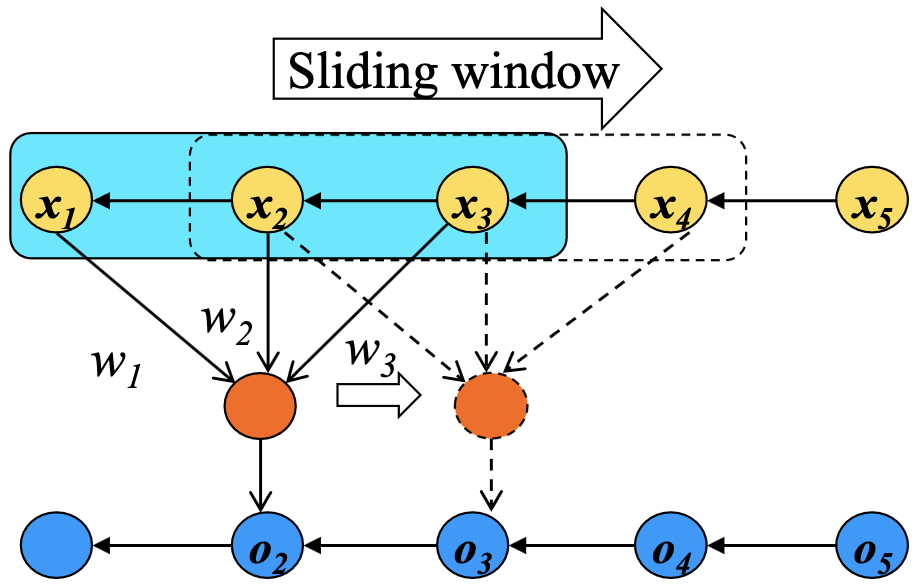
\includegraphics[width=0.45\linewidth]{img/CNN_simple.png}
\end{figure}

Here, the output of each node in the hidden layer is calculated as $out_t = \sum_{i=1}^3 w_i x_{t+i-2}$. In other words, the weights assigned to the inputs ``slide'' across the hidden layer. Weights are tuned as usual by learning.

\subsection{2D Convolution}

Discrete convolution can be seen as a multiplication by a matrix, with several entries constrained to be equal to other entries. The convolution over a 2D image $I$ with a kernel $K$ can be expressed as:
\begin{equation*}
    S(i,j) = (I*K)(i,j) = \sum_m \sum_n I(m,n)K(i-m, j-n) \,,
\end{equation*}
or, as expressed by many libraries, as the \textbf{cross-correlation function}:
\begin{equation*}
    S(i,j) = (I*K)(i,j) = \sum_m \sum_n I(i+m,j+n)K(i, j) \,.
\end{equation*}

The example below shows a 2D image with 25 pixels, and a 3x3 kernel (unit local receptive field) with a stride equal to 1 (i.e., the kernel moves across the image 1 pixel at a time; by choosing the stride we choose the size of the feature map). The image also has padding added to its edge.
\begin{figure}[h]
    \centering
    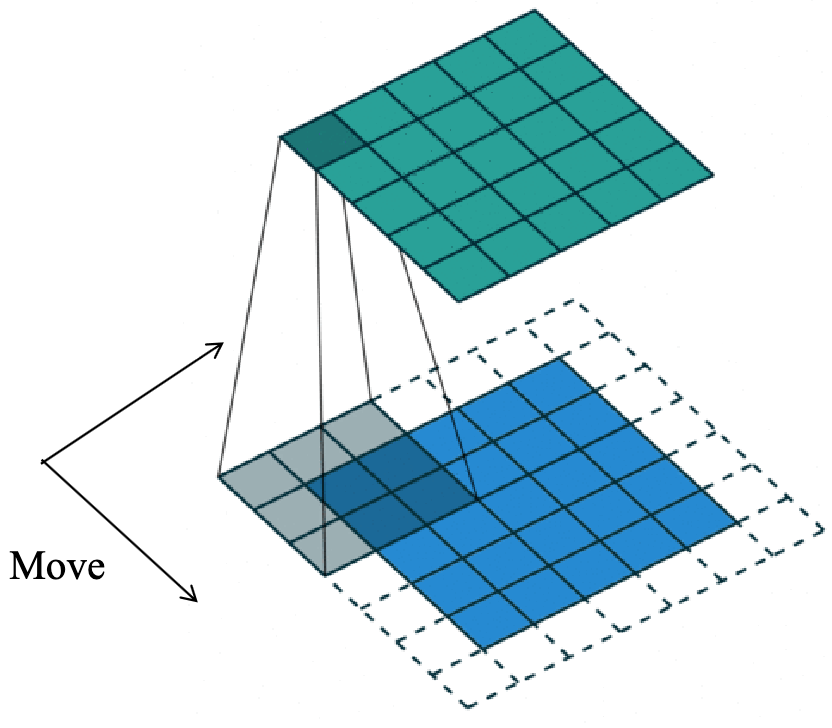
\includegraphics[width=0.6\linewidth]{img/CNN_2D.png} 
\end{figure}

Once the kernel reaches the end of the first ``row'' of pixels, it restarts from the position it started from shifted one pixel below. The full movement of the kernel over the image produces the feature map.

The image below better shows the matrix multiplication interpretation of convolution; the image is 4x3 and the kernel is 2x2. The stride is again equal to 1.

\begin{figure}[h]
    \centering
    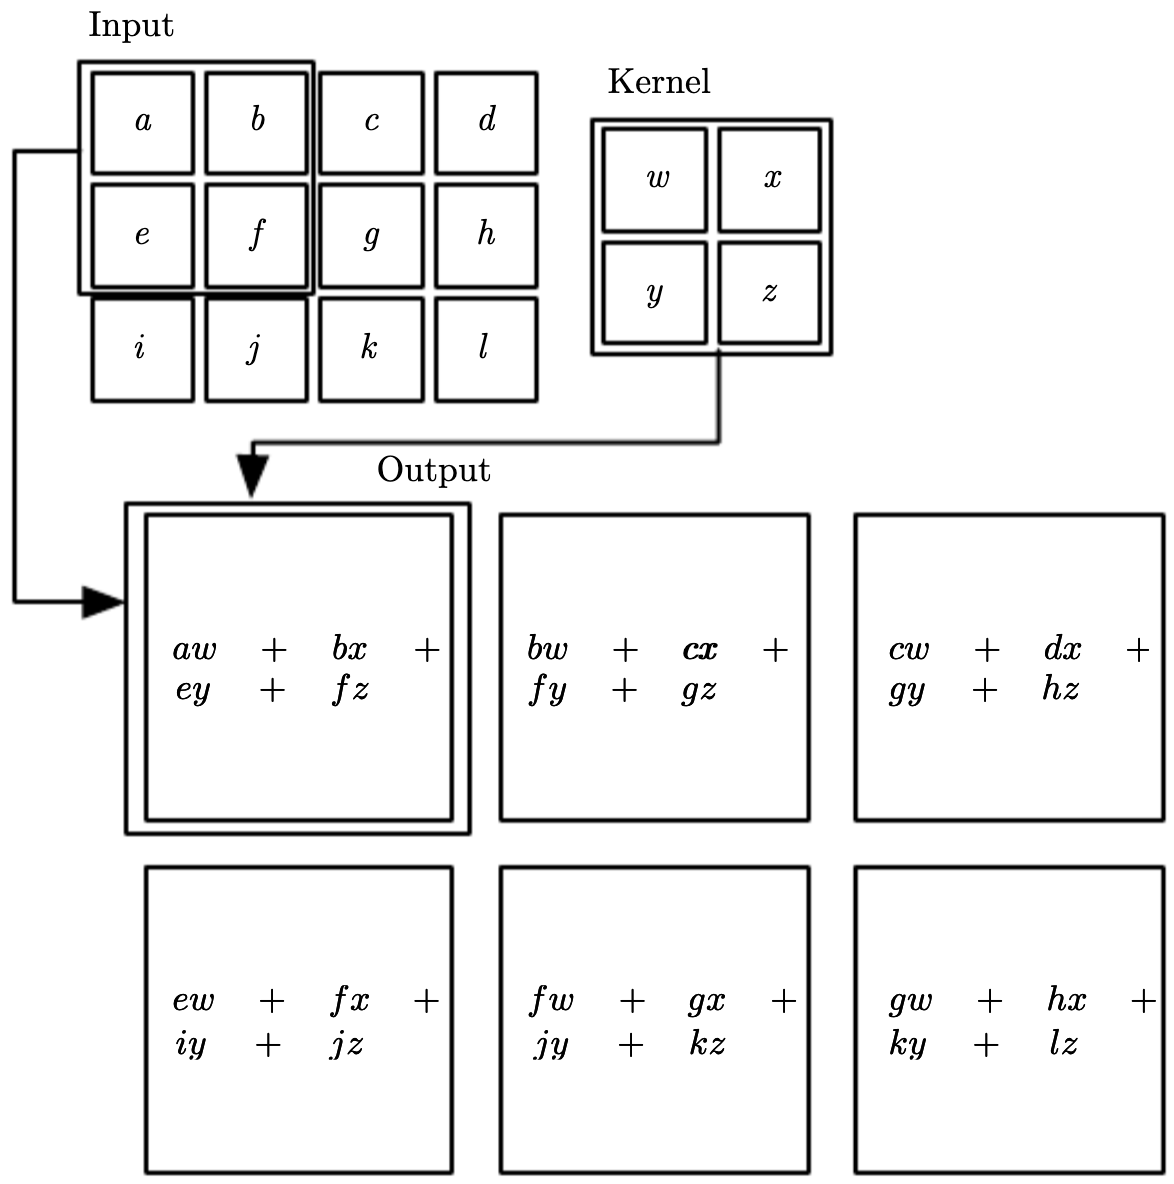
\includegraphics[width=0.5\linewidth]{img/CNN_matrix.png}
\end{figure}
Each unit's weights are a \textbf{filter} trained to detect some specific feature or pattern in the image. Each filter produces the strongest response to a spatially local input pattern, and then the filters obtained by training are applied to the whole (global) image, so that features and patterns can be identified regardless of where they are positioned on the image.

The size of the feature map can be reduced via pooling. Some examples of pooling are:
\begin{itemize}
    \item Subsampling, using a stride greater than 1;
    \item Calculating a mean (average or weighted average);
    \item Using the max pool operation (most common option).
\end{itemize}
This way, instead of producing a value for every single pixel of the original image, we get a smaller set of pixels where each value is obtained by considering the values of neighboring ones (calculating the mean or max value). Pooling also helps to make the representation approximately invariant to small translations of the input, since the mean or max value of a neighborhood of points is unlikely to be affected by a small translation of the pixels in the image.

CNN exploits \textbf{weight sharing}, where the number of connections in the network is kept the same while reducing the number of actual free parameters. The produced sliding window of units is applied over a segment of the input, and reapplied multiple times to produce various layers of feature maps. Training of the weights is usually done via backpropagation. Since these networks tend to be big and deal with large amount of data, many hyperparameters are fixed by experience or by suggestions of experts, since it would be too expensive to run cross-validation.

\section{Deep Learning}

The Deep Learning framework includes many different models, such as:
\begin{itemize}
    \item Deep Neural Networks;
    \item Convolutional Neural Networks;
    \item Deep belief Networks;
    \item Recurrent and Recursive Neural Networks.
\end{itemize}
They differ from ``shallow'' models in that they have a big amount of layers.

There's many different approaches to build a deep learning model. All these approaches have some aspects in common:
\begin{itemize}
    \item Multiple layers of nonlinear processing units;
    \item Supervised or unsupervised learning of feature representation in each layer, with the layers forming some hierarchy from low to high level features;
    \item Hierarchical sparse/distributed representation of the input data.
\end{itemize}

The core concept at the base of deep learning is increasing the level of abstraction of the data through the use of several layers; for example, an image can be gradually abstracted on each layer, first as a vector of intensity values per pixel, then a set of edges, then regions of a particular shape, and so on. We've already mentioned this idea with CNNs: the original complicated mapping is broken down into its simple elements, by gradually calculating simpler mapping at each layer. A series of hidden layers extracts increasingly abstract features from a set of example images. Additionally, these abstract features, once learned by the units, can also be combined together to generalize on examples that were never seen during training.

In general, deeper networks are often able to use less units per layer, thus less free parameters as well and less training data required to achieve a good generalization. Still, many layers may be harder to be trained, so there's a need to improve the techniques we know regarding gradient descent, regularization, and data exploitation.

\subsection{Insights}

\subsubsection{Why So Many Layers?}

Imagine a two-layer circuit of logic gates, which can represent any Boolean function. Any Boolean function can indeed be written as a sum of products (i.e., in disjunctive normal form). With logical circuits of depth two, the number of logic gates required to represent most Boolean functions is exponential w.r.t. input size.

An example of such function is the parity function: it returns 1 if there is an odd number of 1s over $N$ binary inputs (i.e., $N$ bits), 0 otherwise. If we were to implement this function with logic gates, assuming $N$ inputs, we would need:
\begin{equation*}
    \dfrac{2^N}{2} + 1 = 2^{N-1} + 1
\end{equation*}
gates, since we have to perform 1 OR and exactly $2^{N-1}$ ANDs.

We can propose an alternative solution with a polynomial number of gates, by increasing the number of layers to $log(N)$. The solution for $N=8$ is shown below (in a simplified view where each XOR corresponds to 2 AND gates and 1 OR gate). In this solution, the number of gates is greatly reduced from $2^7 + 1 = 129$ to only $7 * 3 = 21$.
\begin{figure}[h]
    \centering
    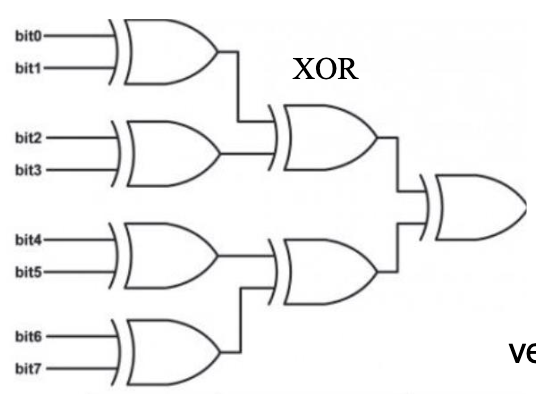
\includegraphics[width=0.5\linewidth]{img/Circuit_deep.png}
\end{figure}

The universal approximation theorem states that even with 1 hidden layer, a NN can approximate any possible function, however it does not specify the number of units needed. For some families of functions a boundary on this number can be found, but as seen in the example above, the bound may be exponential w.r.t. the dimension of the input. Also, there exist families of functions which can be approximated efficiently by a NN with depth greater than some value $d$, but which require a much larger model if depth is restricted to be less or equal than $d$.

This theorem also implies that regardless of what function we are trying to learn, a large MLP is able to represent the function, but there's no guarantee that that the training algorithm will be able to learn that function, either because it can't find the value of the parameters that correspond to the desired function, or because it might choose the wrong function due to overfitting. So another advantage to using multiple layers is ensuring that the learning algorithm can actually properly learn.

The inductive bias is: choosing a deep model encodes the (very general) belief that the function we want to learn should involve composition of several simple functions. If our task actually matches our bias, then the deep shape of the learner is suitable, and those deeper models also perform better than shallow ones. Typically, these tasks are the ones that involve images or language, but for other tasks that deal with different data this deep structure may not be appropriate.

Other challenges that motivate the usage of deep neural networks are related to the curse of dimensionality and manifold learning.

Recall that the curse of dimensionality is the phenomenon in which as the number of dimensions in the data increases, the less dense it is, thus becoming a problem for distance based machine learning algorithms. One challenge posed by this phenomenon is a statistical one: this challenge arises when the number of possible configurations of an input $x$ is much larger than the number of actual training examples. Let's say we want to estimate the probability density for some point $x$ by returning the number of training examples in the same unit volume cell as $x$ divided by the size of the training set. But if we want to estimate this density for a point that has no close neighbors within the unit volume cell (as is often the case when the dimensionality of data is high), there's no immediate way to calculate it. Additionally, even if present, neighbors are likely going to be very few. But deep learning is the solution: it can learn the single features it identifies in the training data, and those features can then be combined to produce an output even for instances that were never seen before.

A manifold is a connected region. Mathematically, it's a set of points associated with a neighborhood around each point. From any given point, the manifold locally appears to be a Euclidean space. As an example, in the real world, we experience the surface of the Earth as 2D, but in reality it's a sphere in 3D space. In the case of Machine Learning, ``manifold'' is a term used to broadly refer to a connected set of points that can be approximated well by considering only a small number of dimensions. Different points can also have a different number of dimensions, typically when the manifold intersects itself. \textbf{Manifold learning} assumes that the only interesting inputs occur only along a collection of manifolds containing a small subset of points, with interesting variations in the output occurring only across directions that lie on the manifold, or only when moving from one manifold to the other. This assumption is often used for data types such as images, text, or audio that occur in real life, since uniform, artificial noise never resembles the inputs from those domains, so the probability distribution of the only valid data is highly concentrated. *?

\subsubsection{Representation Learning}

With Deep Learning, other concepts are emerging, such as representation learning, which is the set of methods that automatically discover the best representation of raw data for some other task. It's especially useful for more complex data types like images, text, or audio data. Deep Learning methods are also representation learning methods with multiple levels of representation.

The reason behind representation learning is that many information processing tasks can have varying difficulty based on the way the information is represented. In Machine Learning, a good representation is one that makes a subsequent learning task easier. Supervised learning in MLPs is an example that leads to an automatic representation at every hidden layer taking on properties that make the output layer task easier (think of the XOR example). Another example is CNNs, since they take as input a raw image and automatically learn to identify the main features of the image, decomposing it into its parts.

The hidden representation of data can be obtained via \textbf{pretraining approaches}, semi-supervised learning, which means we can learn a representation for the unlabeled data and use it to solve supervised tasks. The representation can be then exploited with \textbf{transfer learning} approaches.

\paragraph{Pretraining}

\textbf{Greedy Layer-Wise Unsupervised Pretraining} was the first approach to make it possible to train a deep supervised network. It makes the training of the whole network much easier, since there's no need for an end-to-end training from the output layer to the previous hidden layers with a gradient descent, which used to be difficult for deep models. The adjective ``greedy'' refers to the fact that each layer is optimized independently in an unsupervised way. This methods works not only as a good initialization strategy, but also as regularization regarding the complexity of the original data, since it extracts the features that simplify the unsupervised process. It also reduces the variance of the estimation training process, since pretrained models tend to gather in a smaller region after training).

\paragraph{Autoencoders}

An autoencoder is a neural network that is trained to attempt to copy its input to its output. It has a hidden layer $h$ that describes a \textbf{code} used to represent the input. The network can be seen as two components: the encoder function $h = f(x)$, and the decoder $r = g(h)$ that produces a reconstruction. Autoencoders are specifically trained so that they are unable to copy the input perfectly, but instead only copy parts of the data or copy it only approximately. Since the model is forced to prioritize only some aspects of the input, it often learns useful properties of the data.

Autoencoders can be:
\begin{itemize}
    \item \textbf{Undercomplete}, if the code dimension is less than the input dimension. This autoencoder is forced to learn the salient features of the training data by the constraints in the architecture itself.

    \item \textbf{Overcomplete}, if the code dimension is greater than the input dimension. By itself the autoencoder would learn to copy the input as is, so some form of regularization is needed to introduce constraints in the sparsity of the representation, robustness in the noise, and other properties of interest.
\end{itemize}

A commonly used type of autoencoders are denoising autoencoders. They are trained on a set of images, finding the best representation of them (the one they can obtain even from corrupted/noisy data). Once they are presented with an image with added noise, they are capable of reconstructing the original.

Stacked autoencoders are multiple autoencoders stacked on top of each other. The algorithm used to train a stacked autoencoder is the following:
\begin{enumerate}
    \item Train the first layer as an autoassociator (i.e., an autoecoder whose input and output are the same), in order to minimize the reconstruction error of the raw input;

    \item The hidden units' outputs in the autoassociator are now used as input for another layer, also trained to be an autoassociator. Repeat this step until the desired number of layers is reached.

    \item Take the last hidden layer output as input to a supervised layer, and initialize only its parameters (randomly or by supervised learning).

    \item Fine-tune all the parameters of the architecture with respect to the supervised criterion.
\end{enumerate}

The idea is that the unsupervised greedy layer-wise initialization put all the parameters of all the layers in a region of parameter space from which a local optimum can be reached via local descent.

In the past, pretraining acted as the start of Deep Learning. It can yield improvements for some tasks, especially NLP, but not in others. The general role of pretraining is nowadays under critical revision by researchers.

\paragraph{Transfer Learning}

\textbf{Transfer learning} refer to the situation where what has been learned in one setting is used to improve generalization in another setting. In this case, we use the best representation of the data found by pretraining to improve the generalization capabilities of some model. In \textbf{domain adaptation}, the task remains the same between each setting, but the input distribution is different. With \textbf{multi-task learning}, a trained model can be used for a task that's different from the one it was trained for (it will receive the same inputs, but the target variable(s) change).

\subsubsection{Distributed Representation}

As opposed to \textbf{symbolic representation}, in which each input corresponds to an unique symbol, in \textbf{distributed representation} each input is represented by a set of elements that can be set separately from each other. As an example, consider a vector of $n$ binary features, which can take $2^n$ possible configurations, each corresponding to a different region in input space. This is a type of distributed representation. The same data can be represented via one-hot encoding: $n$ feature detectors, each corresponding to the detection of a certain input. Only $n$ configurations of the input space are possible. This is a type of symbolic representation. The two representations are visualized below.

\begin{table}[h]
    \centering
    \begin{tabular}{|c|cccc|}
        \hline
        \rowcolor{gray}
        Input & barks & hasFur & hasLegs & isFruit \\
        Dog & 1 & 1 & 1 & 0 \\
        Cat & 0 & 1 & 1 & 0\\
        Apple & 0 & 0 & 0 & 1\\
        Kiwi & 0 & 1 & 0 & 1\\
        \hline
    \end{tabular} 
\quad
    \begin{tabular}{|c|cccc|}
        \hline
        \rowcolor{gray}
        Input & isDog & isCat & isApple & isKiwi \\
        Dog & 1 & 0 & 0 & 0 \\
        Cat & 0 & 1 & 0 & 0 \\
        Apple & 0 & 0 & 1 & 0 \\
        Kiwi & 0 & 0 & 0 & 1 \\
        \hline
    \end{tabular}
    \caption{Distributed representation on the left, symbolic representation on the right.}
\end{table}

In distributed representation, values assigned to attributes can also be real-valued. By using this representation, we can calculate similarity between two different concepts (inputs); in symbolic representation, the distance between two inputs is always $\sqrt{2}$.

In general, distributed representation is used in input only if we have background knowledge (one-hot encoding is used instead), while it is commonly used automatically during learning. A big advantage is that there's no need to characterize all the possible configurations of the input, but only the distinction across specific concepts (e.g., in the example above, we learn the characteristics ``barks'', ``hasFur'', ``isFruit'' instead of learning exactly what a dog or an apple are).

Sharing attributes among inputs allows the model to both treat them similarly, and automatically learn such similarity. As per the example above, ``dog'' and ``cat'' share some features. If we are presented with textual data containing several different words, and by learning the model knows the similarity between ``cat'' and ``dog'', a sentence that contains the word ``cat'' can inform the predictions made for a sentence containing the word ``dog'', and vice-versa. Since they're represented in a distributed way, the distance between the two is actually measurable and comparable with respect to other inputs (e.g., ``dog'' is closer to ``cat'' but both are further away from ``apple'', while with one-hot-encoding their distance is $\sqrt{2}$ regardless of how similar the concepts represented by those words are).

One drawback of distributed representation is that it's more difficult to interpret.

\subsection{Techniques}

When implementing a deep neural network, there's many technical aspects to consider. As already stated before, the deeper the network, the less units are needed for each layer, and therefore there will be less parameters to train, but some layers may be difficult to train. This section will focus on the methods that need improvement and their issued when used with deep NNs.

The first issue is related to the gradient. With deep NNs, there's now a lot of layers to backpropagate the gradient through. If the weights are too small, they will shrink exponentially (gradient vanish), while if they are too big, they will grow exponentially. This happens because the repetition of multiplication through many layers can introduce cliffs in the cost functions, that when traversed will drastically increase or decrease the weights. One solution is using \textbf{gradient clipping}: if the norm of the gradient $\|g\|$ is greater than some threshold $v$, then $g = v*\frac{g}{\|g\|}$, so the movement towards the gradient direction still happens, but the weight updates are bounded.

For gradient vanish, traditional activation functions have gradients in the range $[-1,1]$, and backpropagation computes gradients via chain rule repeated through layers. This means that for each layer, the gradient of the layer in the front will be multiplied by a value $d,\,|d| \geq 1$, so the layers closer to the input will be trained much more slowly. There are many approaches to deal with it, one of which is using the \textbf{ReLU (Rectified Linear Unit)} activation function:
\begin{equation*}
    f(x) = \max(0,x)
\end{equation*}
This function makes it so that the derivative of a unit remains large as long as the unit is active. *?

\textbf{Batch normalization} is a method that normalizes each batch by calculating each individual batch statistics such as mean and variance for each layer. Each matrix (batch x activation of units) is normalized with mean and variance, shifting the values to zero-mean and unit variance. This technique helps to keep the normalization of the input across all layers of the network. It also achieves a faster learning and higher accuracy for Deep Learning.

\textbf{Dropout} is a method that makes bagging more practical for large neural networks. Bagging involves training multiple models on different subsets of the data, and then evaluating multiple models on the same test example. Dropout trains the ensemble consisting of all sub-networks that can be formed by removing non-output units from an underlying base network. In most modern neural networks, we can effectively remove a unit from a network by multiplying its output value by 0. Then, a minibatch-based learning algorithm is used to train one working sub-network at a time. The sub-network is selected at random, with each binary mask to apply to the original network having a different probability set as an hyperparameter (e.g., 0.8 for input units and 0.5 for hidden units). The sub-networks inevitably share weights, since they're obtained from the same base network; this causes the training of the sub-networks to find good settings for the parameters.

Dropout has a regularization effect as well: it avoids to train all units on all training data and reduces unit interactions. It also reduces variance without affecting bias just like bagging does. It even regularizes singular hidden units to be not just good features, but features that can be good in different contexts (different sub-networks). It can be used for any model that uses distributed representation and SGD training.